% Model report generated by SolverMapp.
% Compile with: pdflatex, bibtex, pdflatex, pdflatex (references.bib is written by the first run).
\begin{filecontents*}[overwrite]{references.bib}
@misc{ref,
  note   = {Index notation test},
  key    = {Index notation test}
}
\end{filecontents*}
\documentclass[11pt,a4paper]{article}
\usepackage[T1]{fontenc}
\usepackage[utf8]{inputenc}
\usepackage{lmodern}
\usepackage{amsmath,amssymb}
\usepackage{booktabs,longtable}
\usepackage{siunitx}
\usepackage{algorithm}
\usepackage{algpseudocode}
\usepackage{tikz}
\usetikzlibrary{positioning,shapes.geometric,shapes.misc,arrows.meta}
\usepackage{adjustbox}
\usepackage[hidelinks]{hyperref}

\title{Matrices in index notation: Hilbert matrix, products, sums}
\author{}
\date{\today}

\begin{document}
\maketitle

The model consists of 6 equations in 8 variables: 2 inputs, 0 state variables, 2 intermediate variables and 4 outputs. It is solved in 3 steps (Algorithm~\ref{alg:solution}).

\section{Nomenclature}
\begin{longtable}{@{}l p{0.48\linewidth} l l@{}}
  \toprule
  Symbol & Description & Unit & Value \\
  \midrule
  \endhead
  \bottomrule
  \endfoot
  \multicolumn{4}{@{}l}{\textit{Inputs}} \\
  $Q$ & Second matrix (identity) & -- & I \\
  $n$ & Size & -- & \num{6} \\
  \addlinespace
  \multicolumn{4}{@{}l}{\textit{Intermediate variables}} \\
  $H$ & Hilbert matrix & -- &  \\
  $b$ & Row sums & -- &  \\
  \addlinespace
  \multicolumn{4}{@{}l}{\textit{Outputs}} \\
  $\mathbf{x}$ & Solution (all ones) & -- &  \\
  $C$ & H B & -- &  \\
  $\tau$ & Trace & -- &  \\
  $d$ & Partial column sums & -- &  \\
\end{longtable}

\section{Governing equations}

\subsection{Hilbert matrix}
Source: \cite{ref}, Eq.~(1).
\begin{equation}
  H_{ij} = \frac{1}{i + j - 1}
  \label{eq:hilbert-matrix}
\end{equation}
\noindent where

\noindent\begin{tabular}{@{\quad}l@{\quad}p{0.7\linewidth}@{}}
  $H$ & Hilbert matrix, dimensionless \\
\end{tabular}

\noindent Holds for every $i = 1, \dots, n$ and $j = 1, \dots, n$.

\subsection{Row sums}
Source: \cite{ref}, Eq.~(2).
\begin{equation}
  b_i = \sum_j H_{ij}
  \label{eq:row-sums}
\end{equation}
\noindent where

\noindent\begin{tabular}{@{\quad}l@{\quad}p{0.7\linewidth}@{}}
  $b$ & Row sums, dimensionless \\
  $H$ & Hilbert matrix, dimensionless \\
\end{tabular}

\noindent Holds for every $i = 1, \dots, n$.

\subsection{Product}
Source: \cite{ref}, Eq.~(4).
\begin{equation}
  C_{ij} = \sum_k H_{ik} Q_{kj}
  \label{eq:product}
\end{equation}
\noindent where

\noindent\begin{tabular}{@{\quad}l@{\quad}p{0.7\linewidth}@{}}
  $C$ & H B, dimensionless \\
  $H$ & Hilbert matrix, dimensionless \\
  $Q$ & Second matrix (identity), dimensionless \\
\end{tabular}

\noindent Holds for every $i = 1, \dots, n$ and $j = 1, \dots, n$.

\subsection{Trace}
Source: \cite{ref}, Eq.~(5).
\begin{equation}
  \tau = \sum_i H_{ii}
  \label{eq:trace}
\end{equation}
\noindent where

\noindent\begin{tabular}{@{\quad}l@{\quad}p{0.7\linewidth}@{}}
  $\tau$ & Trace, dimensionless \\
  $H$ & Hilbert matrix, dimensionless \\
\end{tabular}


\subsection{Shifted}
Source: \cite{ref}, Eq.~(6).
\begin{equation}
  d_i = \sum_{j=1}^{i} H_{j1}
  \label{eq:shifted}
\end{equation}
\noindent where

\noindent\begin{tabular}{@{\quad}l@{\quad}p{0.7\linewidth}@{}}
  $d$ & Partial column sums, dimensionless \\
  $H$ & Hilbert matrix, dimensionless \\
\end{tabular}

\noindent Holds for every $i = 1, \dots, n$.

\subsection{Solve}
Source: \cite{ref}, Eq.~(3).
\begin{equation}
  \mathbf{x} = H^{-1} b
  \label{eq:solve}
\end{equation}
\noindent where

\noindent\begin{tabular}{@{\quad}l@{\quad}p{0.7\linewidth}@{}}
  $\mathbf{x}$ & Solution (all ones), dimensionless \\
  $H$ & Hilbert matrix, dimensionless \\
  $b$ & Row sums, dimensionless \\
\end{tabular}


\section{Solution algorithm}
\begin{algorithm}[htbp]
  \caption{Solution procedure}\label{alg:solution}
  \begin{algorithmic}[1]
    \State Set the inputs $Q$ and $n$
    \State Compute $H$ for every $i$ and $j$ from Eq.~\eqref{eq:hilbert-matrix}
    \State Compute $b$ for every $i$ from Eq.~\eqref{eq:row-sums}
    \State Compute $C$ for every $i$ and $j$ from Eq.~\eqref{eq:product}
    \State Compute $\tau$ from Eq.~\eqref{eq:trace}
    \State Compute $d$ for every $i$ from Eq.~\eqref{eq:shifted}
    \State Compute $\mathbf{x}$ from Eq.~\eqref{eq:solve}
  \end{algorithmic}
\end{algorithm}

Figure~\ref{fig:flowchart} shows the same procedure as a flowchart.

\begin{figure}[htbp]
  \centering
  \begin{adjustbox}{max width=\linewidth, max totalheight=0.9\textheight}
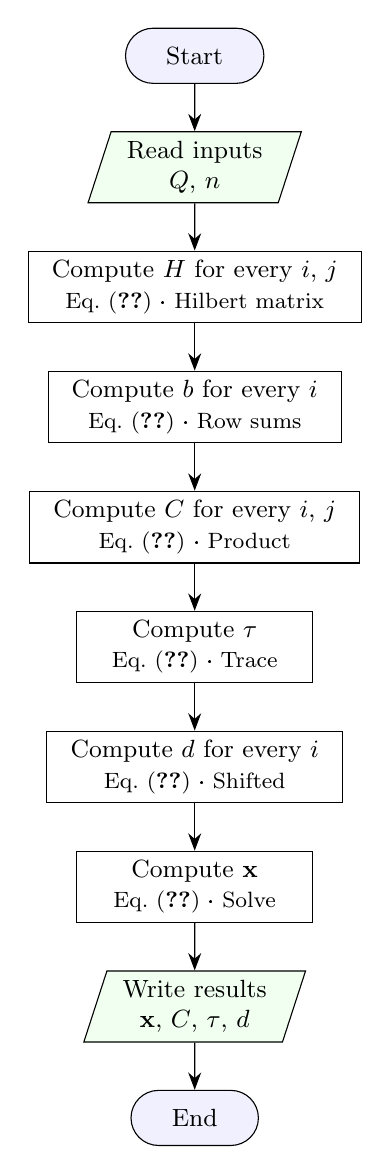
\begin{tikzpicture}[
  node distance=6mm, >={Stealth[length=2.2mm]}, font=\small,
  every node/.style={align=center},
  term/.style={draw, rounded rectangle, minimum height=7mm, inner xsep=5mm, fill=blue!6},
  io/.style={draw, trapezium, trapezium left angle=72, trapezium right angle=108, trapezium stretches body, minimum height=8mm, inner xsep=2mm, fill=green!6},
  proc/.style={draw, rectangle, minimum height=8mm, minimum width=30mm, inner xsep=3mm},
  dec/.style={draw, diamond, aspect=2.4, inner sep=1pt, fill=orange!8},
  lbl/.style={font=\footnotesize, inner sep=2pt}]
  \node[term] (n1) {Start};
  \node[io, below=of n1] (n2) {Read inputs \\ $Q$, $n$};
  \node[proc, below=of n2] (n3) {Compute $H$ for every $i$, $j$ \\ {\footnotesize Eq.~\eqref{eq:hilbert-matrix} \textperiodcentered{} Hilbert matrix}};
  \node[proc, below=of n3] (n4) {Compute $b$ for every $i$ \\ {\footnotesize Eq.~\eqref{eq:row-sums} \textperiodcentered{} Row sums}};
  \node[proc, below=of n4] (n5) {Compute $C$ for every $i$, $j$ \\ {\footnotesize Eq.~\eqref{eq:product} \textperiodcentered{} Product}};
  \node[proc, below=of n5] (n6) {Compute $\tau$ \\ {\footnotesize Eq.~\eqref{eq:trace} \textperiodcentered{} Trace}};
  \node[proc, below=of n6] (n7) {Compute $d$ for every $i$ \\ {\footnotesize Eq.~\eqref{eq:shifted} \textperiodcentered{} Shifted}};
  \node[proc, below=of n7] (n8) {Compute $\mathbf{x}$ \\ {\footnotesize Eq.~\eqref{eq:solve} \textperiodcentered{} Solve}};
  \node[io, below=of n8] (n9) {Write results \\ $\mathbf{x}$, $C$, $\tau$, $d$};
  \node[term, below=of n9] (n10) {End};
  \draw[->] (n1) -- (n2);
  \draw[->] (n2) -- (n3);
  \draw[->] (n3) -- (n4);
  \draw[->] (n4) -- (n5);
  \draw[->] (n5) -- (n6);
  \draw[->] (n6) -- (n7);
  \draw[->] (n7) -- (n8);
  \draw[->] (n8) -- (n9);
  \draw[->] (n9) -- (n10);
\end{tikzpicture}
  \end{adjustbox}
  \caption{Flowchart of the solution procedure}\label{fig:flowchart}
\end{figure}

\bibliographystyle{plain}
\bibliography{references}

\end{document}